\documentclass[12pt]{report}
\linespread{1.3}

\usepackage[utf8]{inputenc}
\usepackage[T1]{fontenc}
\usepackage{xcolor}
\usepackage{inconsolata} % font type

\usepackage{lmodern}
\usepackage{graphicx}
% \graphicspath{ {figure/} }

\usepackage{t1enc}

\definecolor{pblue}{rgb}{0.13,0.13,1}
\definecolor{pgreen}{rgb}{0,0.5,0}
\definecolor{pred}{rgb}{0.9,0,0}
\definecolor{pgrey}{rgb}{0.46,0.45,0.48}
\definecolor{plightgrey}{rgb}{0.94,0.94,0.96}
\definecolor{pmagenta}{rgb}{0.15,0.37,0.46}
\definecolor{pgreen2}{rgb}{0.15,0.37,0.46}

\usepackage{listings}
\lstset{
  captionpos=b,
  showspaces=false,
  showtabs=false,
  breaklines=true,
  showstringspaces=false,
  breakatwhitespace=true,
  commentstyle=\color{pgreen},
  keywordstyle=\color{pblue},
  stringstyle=\color{pred},
  basicstyle=\ttfamily,
  moredelim=[il][\textcolor{pgrey}]{$$},
  moredelim=[is][\textcolor{pgrey}]{\%\%}{\%\%},
  basicstyle=\footnotesize,
  frame=single,
  numbers=left,
  stepnumber=1,
  showstringspaces=false,
  tabsize=1,
  breaklines=true,
  breakatwhitespace=false,
  backgroundcolor=\color{plightgrey}
}

\lstset{basicstyle=\ttfamily\footnotesize,breaklines=true}

% \usepackage{csquotes}
% \usepackage[magyar]{babel}
\usepackage[backend=biber]{biblatex}
\usepackage{geometry}
\geometry{
 a4paper,
 total={160mm,247mm},
 left=25mm,
 top=25mm,
}

\usepackage{titlesec}
\newcommand{\hsp}{\hspace{15pt}}
\titleformat{\chapter}[hang]{\normalfont\Huge\bfseries}{\arabic{chapter} \hsp\color{lightgray}|\hsp}{1ex}{}
\titlespacing*{\chapter}{0pt}{-30pt}{30pt}

\usepackage{hyperref}

\bibliography{ref.bib}

\begin{document}

\thispagestyle{empty}
\begin{center}

{\Huge\bf Data Warehouses and Big Data\newline Final project}\\
\vspace{2.5cm}
{\Large\bf Attila Ambrus} \\
\vspace{0.5cm}
{\small Computer Scientist\\BSc student}\\
\vspace{1cm}
Coimbra, 2024
\vspace{1.5cm}


\end{center}


\thispagestyle{empty}
\clearpage
\pagenumbering{arabic}

\chapter{Introduction}
A data warehouse is a centralized repository designed to store, manage, and analyze large volumes of structured and semi-structured data from multiple sources. Unlike traditional databases, which are optimized for transaction processing, data warehouses are optimized for querying and reporting, making them an essential component in business intelligence and analytics.

The primary function of a data warehouse is to provide a cohesive and consistent data source for decision-making processes. It integrates data from various operational systems, such as customer relationship management (CRM), enterprise resource planning (ERP), and other internal and external data sources, transforming it into a unified format. This integration enables organizations to perform complex queries and generate reports, dashboards, and visualizations that support strategic planning and operational improvements.

Data warehouses employ a variety of techniques to ensure data integrity, accuracy, and accessibility. These techniques include data cleaning, transformation, and loading (ETL), as well as the use of schemas such as star and snowflake to organize data in a way that optimizes performance. Modern data warehouses also leverage advanced technologies such as cloud computing, in-memory processing, and machine learning to enhance scalability, speed, and analytical capabilities.

The evolution of data warehousing has paralleled advancements in technology, leading to the development of data lakes and hybrid models that can handle unstructured data and support real-time analytics. As organizations increasingly rely on data-driven insights to gain a competitive edge, the role of data warehouses continues to expand, making them a cornerstone of modern data architecture.

\chapter{Tools}

\section{Docker}

Docker is an open-source platform designed to automate the deployment, scaling, and management of applications using containerization. Containers are lightweight, portable units that package an application and its dependencies together, ensuring consistent behavior across different environments.

That is why I chose to create my project in a Docker environment. I created a docker-compose file, for pgAdmin, and postgresql. For initializing the database, and configuring pgAdmin, I mount the appropriate files in the containers, as both of these offer configurating them via config files.
The frontentd application was created with sveltekit. I tryed to use Radzen, as suggested but sadly it crashed on my computer. For the frontend application I created a Dockerfile, so the docker compose can manage this part of the project too.

\section{ERDPlus}

ERDPlus is an online tool for creating entity-relationship diagrams (ERDs), relational schemas, star schemas, and other database design diagrams. It is user-friendly and provides a drag-and-drop interface, making it easy for users to visually design and document their database structures. ERDPlus supports the creation of detailed diagrams that represent the data models and relationships within a database, facilitating better understanding and communication among developers, analysts, and stakeholders. This tool is particularly useful for designing databases from scratch, but when I needed to change some things in the schema, doing it through ERDPlus would be more work. It was good to make the base schema, but for only that.

\section{PostgreSQL}

PostgreSQL, often referred to as Postgres, is a powerful, open-source relational database management system (RDBMS). Known for its robustness, extensibility, and standards compliance, PostgreSQL supports a wide range of data types and advanced features such as transactions, foreign keys, subqueries, triggers, and views. It also includes support for JSON and XML, allowing it to handle both structured and semi-structured data. PostgreSQL is highly customizable and extensible, offering numerous extensions for full-text search, geospatial data (PostGIS), and more. Its strong community support and comprehensive documentation make it a popular choice for developers and organizations needing a reliable and versatile database solution.



\section{pgAdmin}

pgAdmin is an open-source management and administration tool for PostgreSQL. It provides a graphical interface that simplifies the tasks of database administration, including creating databases, running queries, managing users and permissions, and monitoring database performance. pgAdmin supports multiple PostgreSQL versions and offers features like SQL query editor, debugging tools, and data visualization capabilities. It is available as a desktop application and a web-based tool, making it accessible from various platforms and devices.

I only used the query tool in pgAdmin, but it was a nice experience.

\section{Radzen}

Radzen is a low-code, rapid application development platform that enables users to build web applications with minimal coding effort.

Sadly I couldn't use it, because it crashed when I tried to connect the database. I didn't like, that I couldn't specify the port number of the database.

\section{SvelteKit}

SvelteKit is a modern framework for building web applications that leverages the power of Svelte, a popular front-end JavaScript framework. Unlike traditional frameworks that use a virtual DOM, Svelte compiles components into highly efficient imperative code that directly manipulates the DOM. SvelteKit extends this approach by providing a comprehensive set of tools for building full-stack applications, including file-based routing, server-side rendering (SSR), and static site generation (SSG). It aims to offer a seamless developer experience with fast performance, simplified state management, and minimal boilerplate code, making it an attractive choice for developers looking to create dynamic, high-performance web applications.

It's the frontend framework that I am most familiar with, thats why I choose to use it.

\subsubsection{Chart.js}
Chart.js is a popular open-source JavaScript library for creating dynamic, responsive, and customizable charts and graphs. Designed to be simple and flexible, it enables developers to easily integrate a variety of chart types, including line, bar, radar, pie, polar area, doughnut, and bubble charts, into web applications. With its intuitive API and extensive documentation, Chart.js allows for the straightforward visualization of data, making it a valuable tool for data analysis and presentation. It also supports animations and interactions, enhancing the user experience and providing clear, visually appealing representations of complex data sets. 

When I shearched for js diagram libraries this was the most appealing to me, that's why I choose to use this.


\chapter{Implementation} % (fold)

\section{ETL}

\begin{figure}[!ht]  
    \begin{center}
        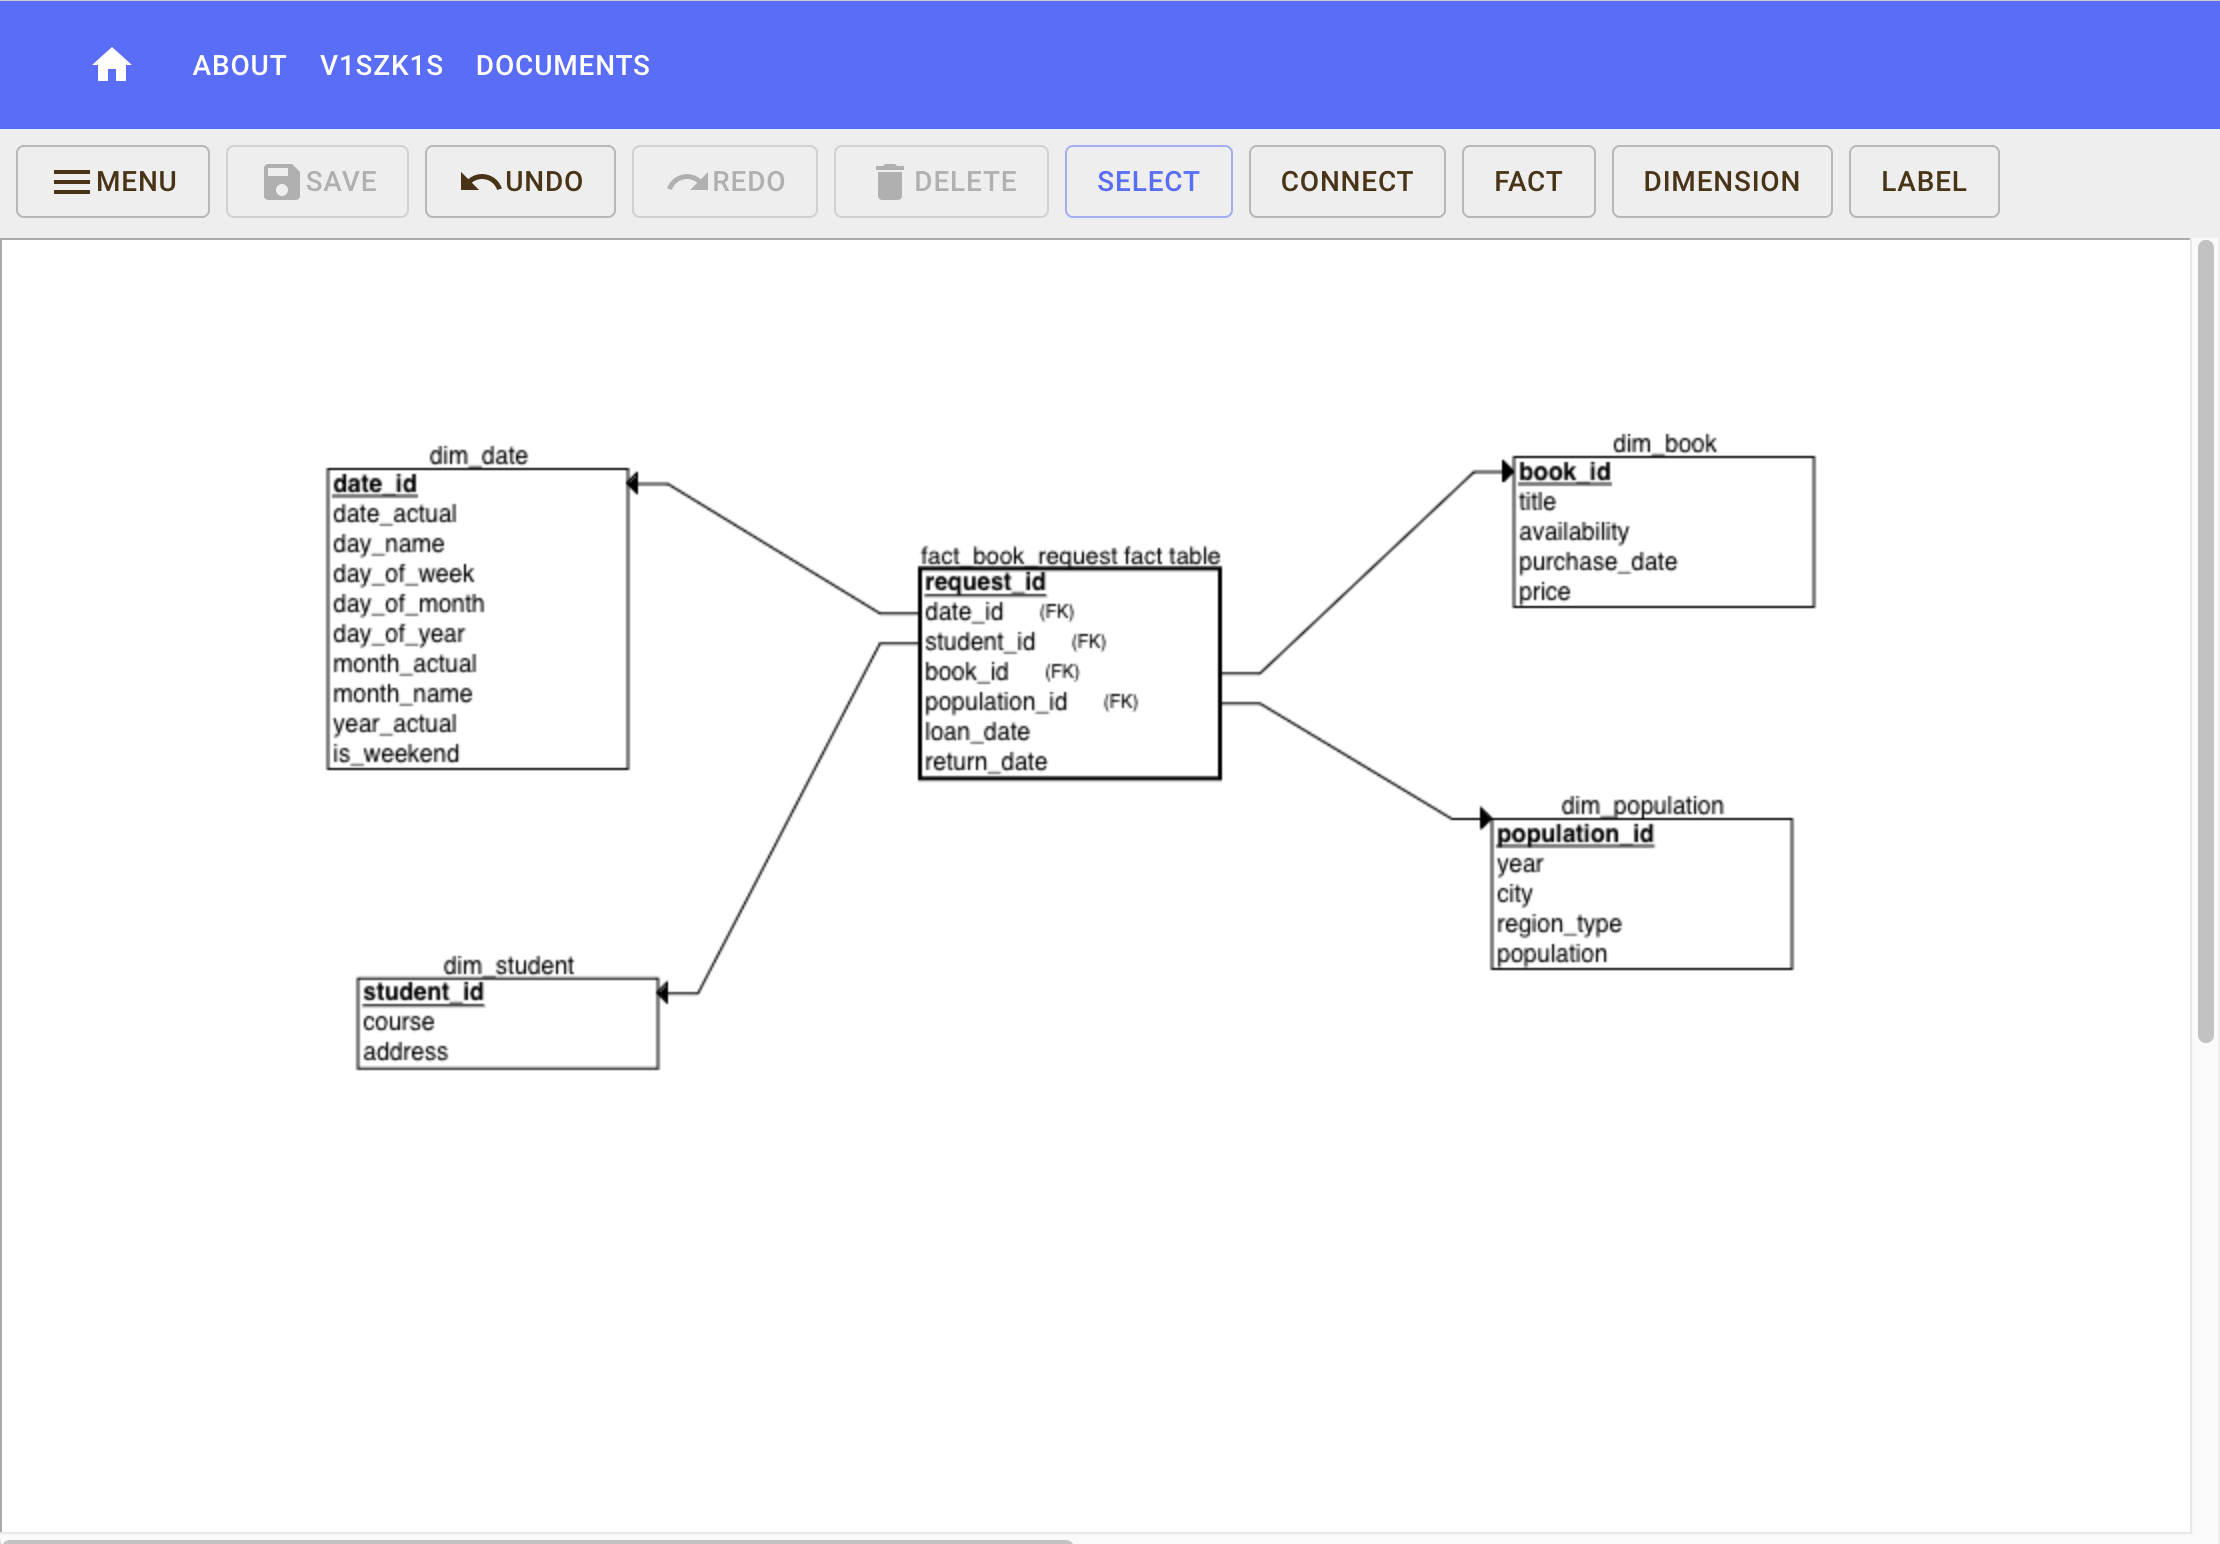
\includegraphics[width=0.95\textwidth]{figures/erd_schema.png}
    \end{center}
    \caption{ERDPlus Schema}\label{fig:schema}
\end{figure}

ETL stands for Extract, Transform and Load. The provided csv files were far from usable format. Frist I needed to filter the neccessary rows, and I also had to obtain the maximum length of some of the attributes.
The ids of the books differed in the provided csvs, so I changed the uniq ids of the books to integers in the range, that the requesests.csv file had.

I sketched the star shcema of the Data Warehouse using ERDPlus. A payed attention to use the appropriate types, as seen in Figure~\ref{fig:schema} 

After creating the schema using drag and drop features, which I find not so pleasent to use, I exported the sql file that the ERDPlus generated for me from the scema as seen on Figure~\ref{fig:erd_sql}.

I would also mention, that after the initial generated sql schema I had to change the init file numerous times.

\begin{figure}
    \begin{center}
        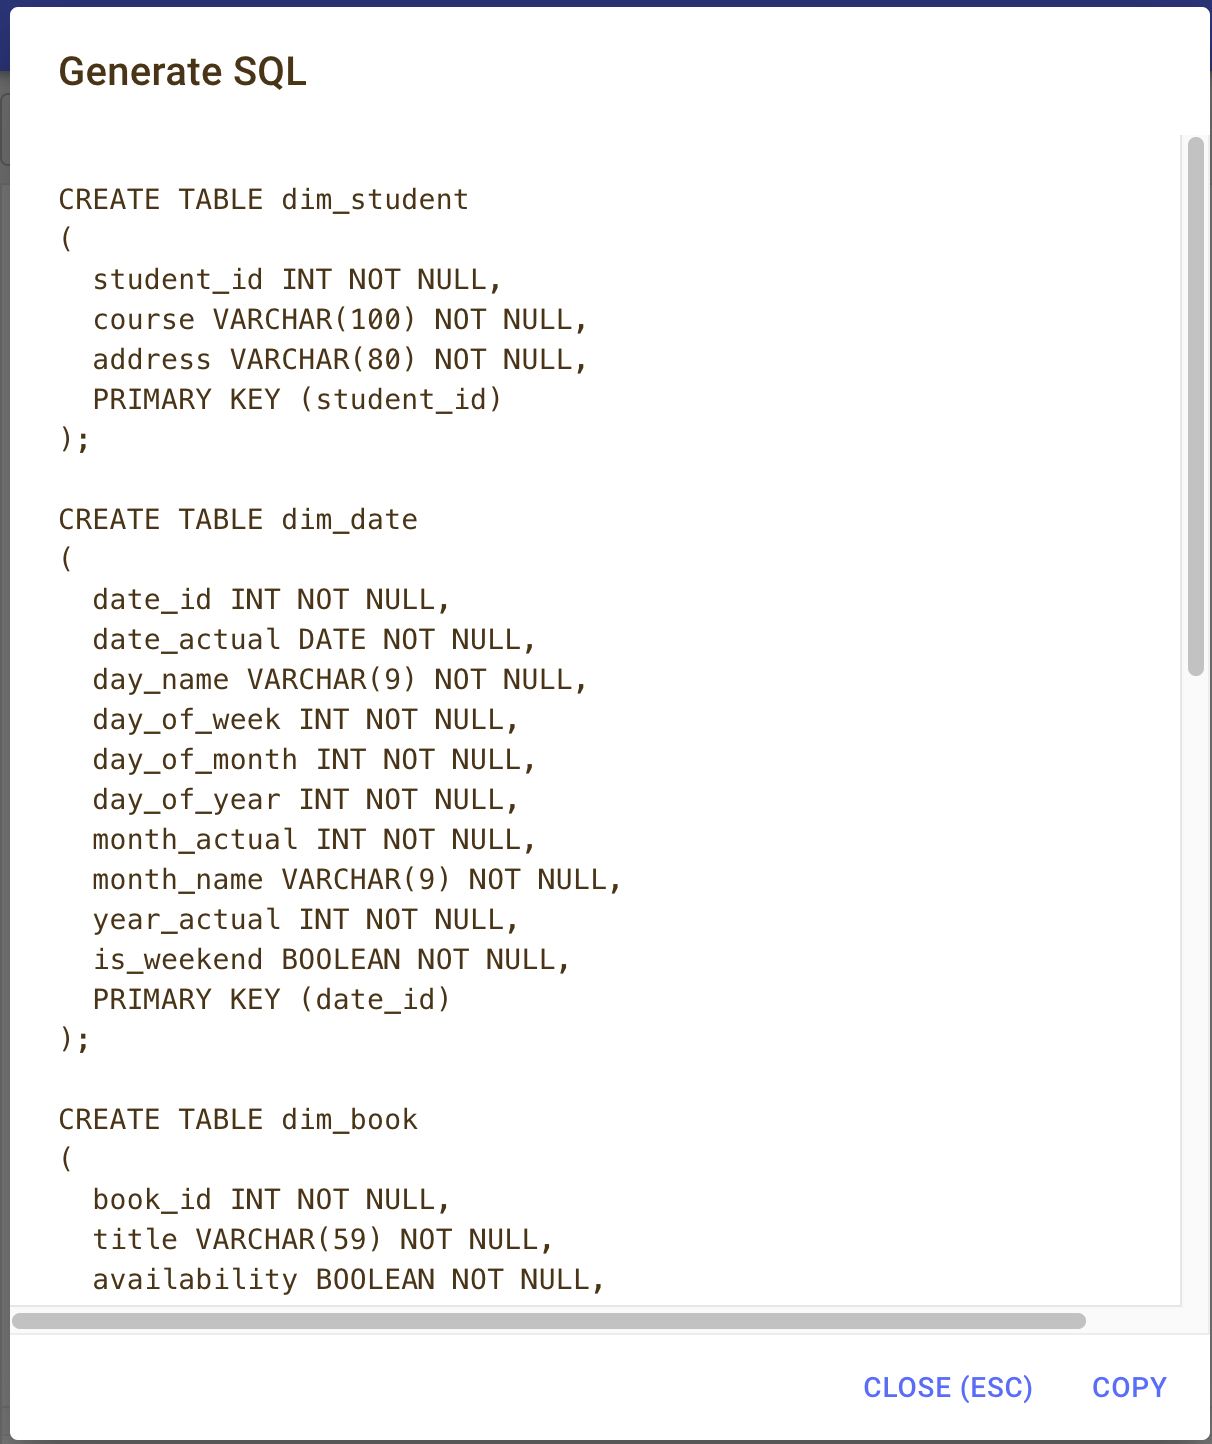
\includegraphics[width=0.95\textwidth]{figures/erd_sql.png}
    \end{center}
    \caption{ERDPlus Generated SQL}\label{fig:erd_sql}
\end{figure}


Now I was ready to import the data from the csv files. The initializing sql file can be seen at Appendix~\ref{appendix:init_sql}.
I mainly used pgAdmin to interact with the database. pgAdmin has a nice user interface where we can see the results of a query \ref{fig:pg_admin_query}.

I, then created all the queries and the views to answer the questions.

\begin{figure}
    \begin{center}
        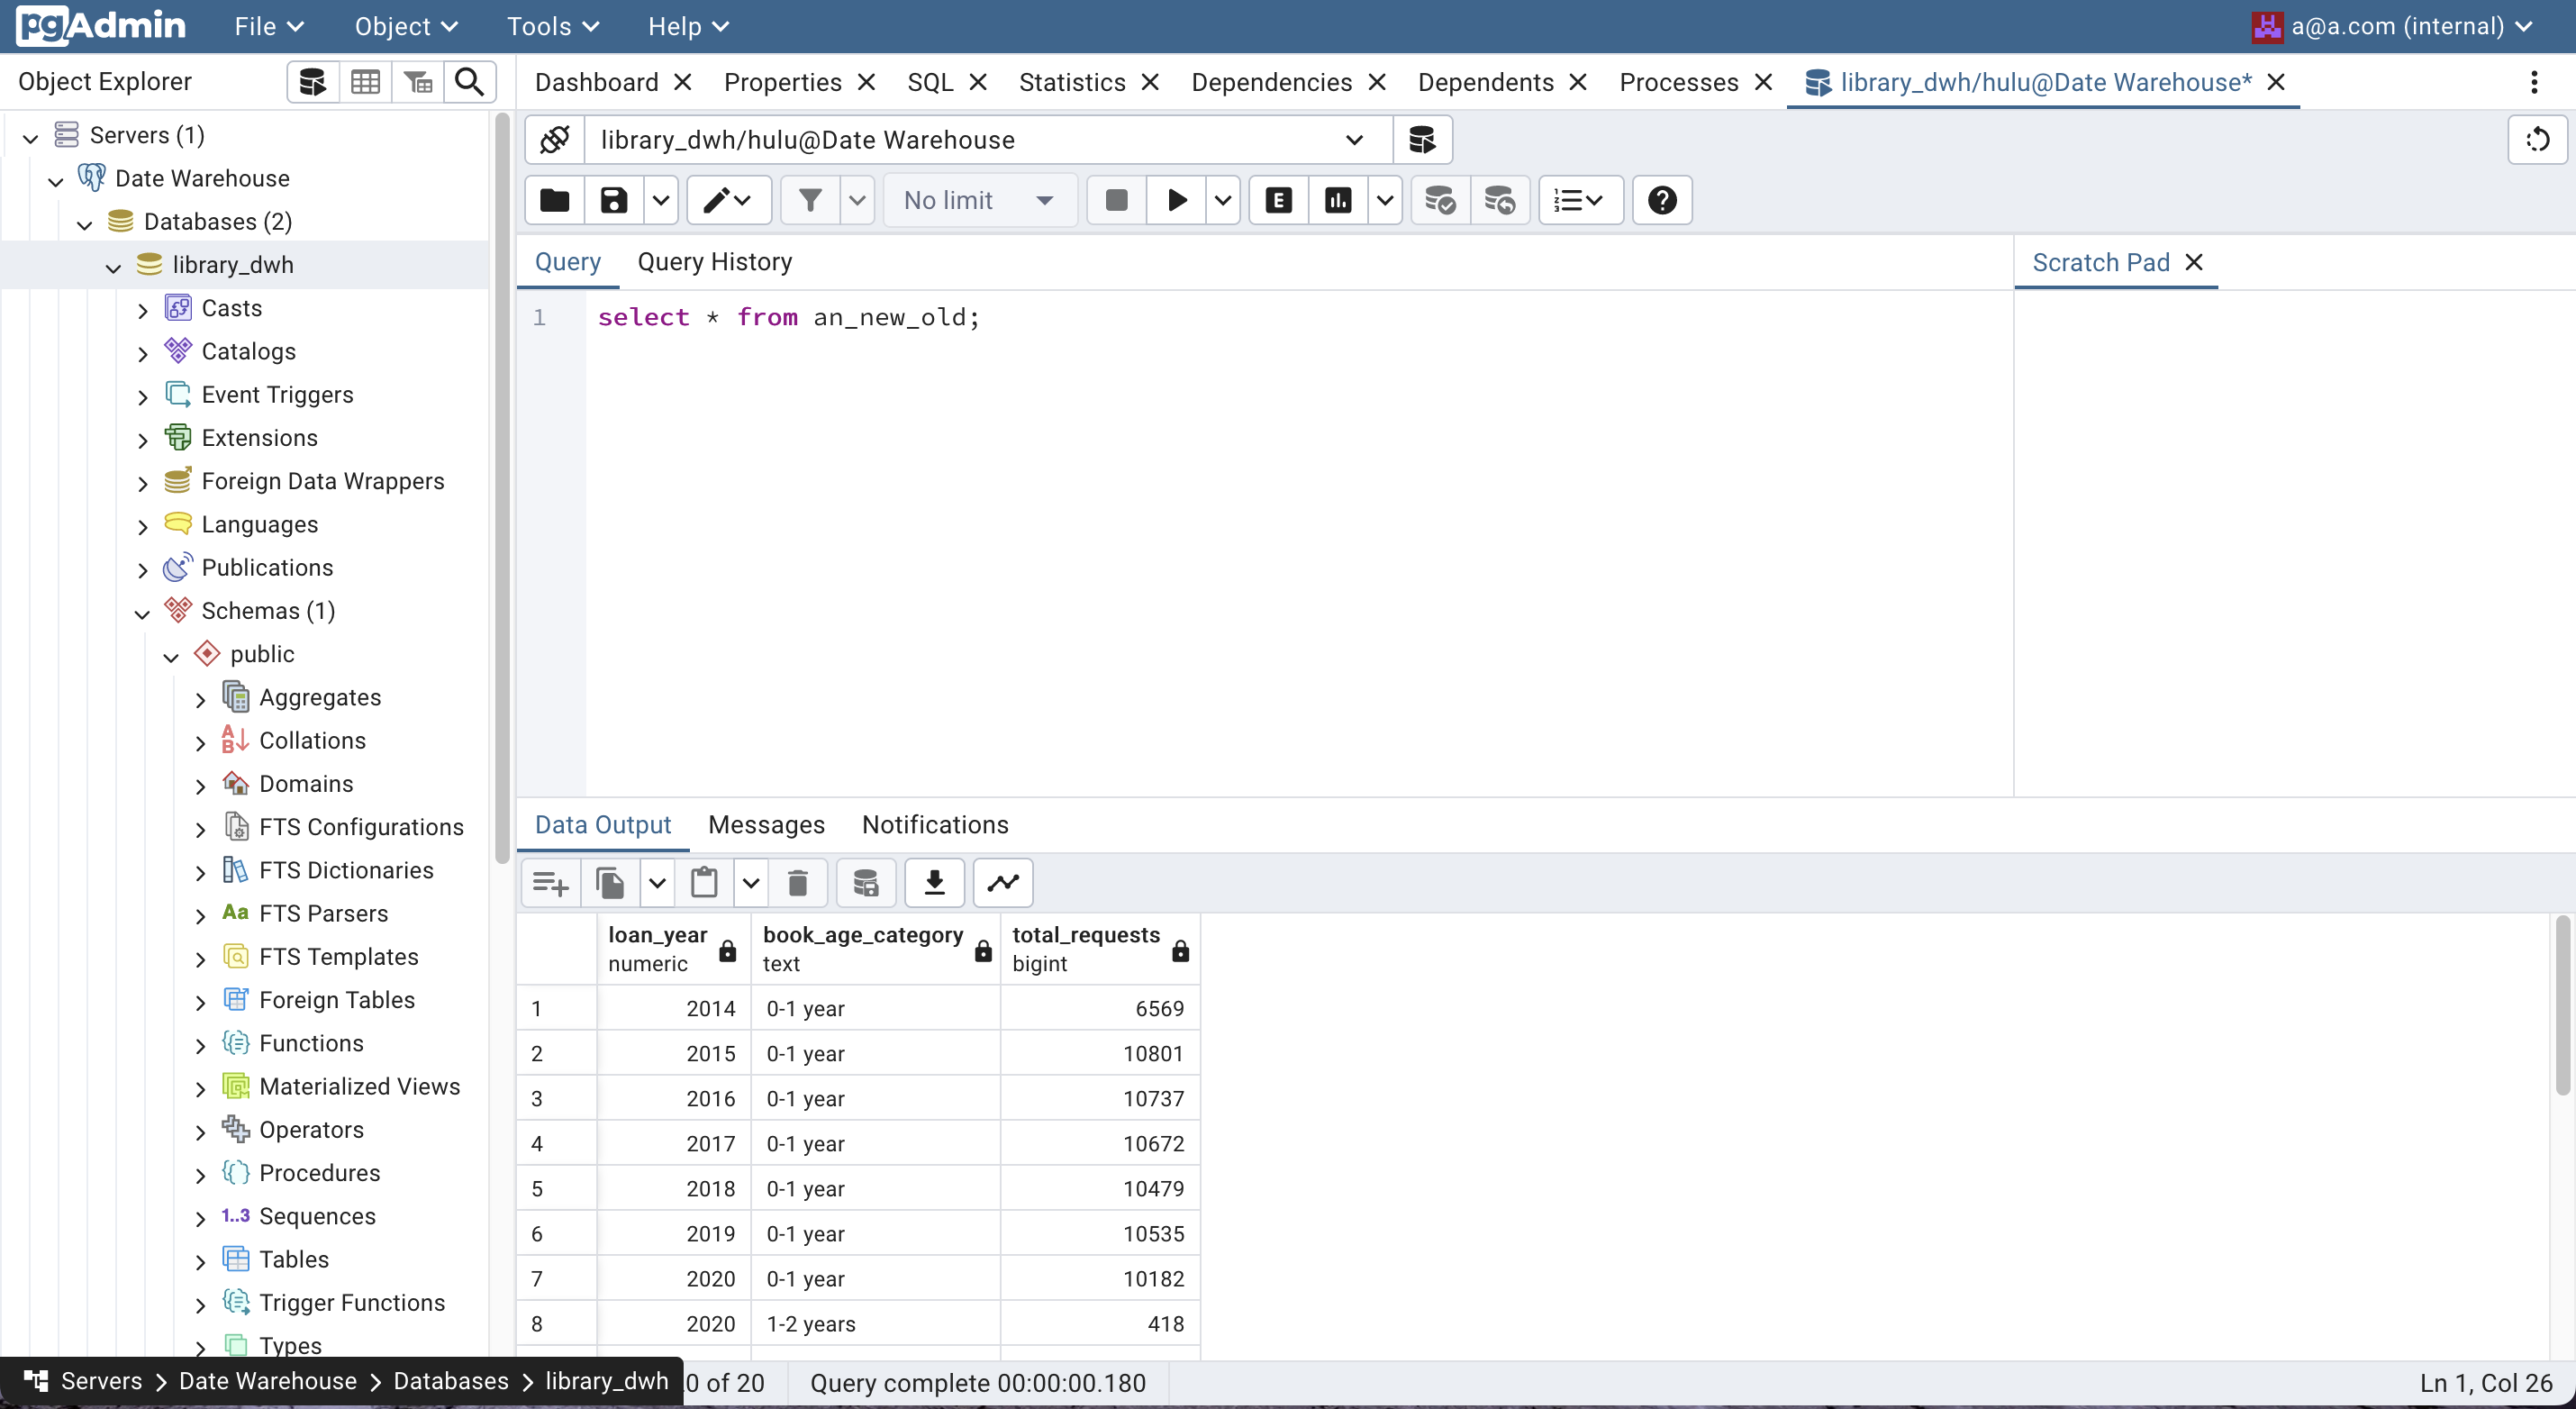
\includegraphics[width=0.95\textwidth]{figures/pg_admin_query.png}
    \end{center}
    \caption{pgAdmin Querying Interface}\label{fig:pg_admin_query}
\end{figure}


\section{Fronted Application}

As part of the final project for the data warehouses class, we were tasked with developing a frontend application to visualize the results of various queries and analyses in chart form. Originally, the requirement was to use the Radzen tool for this purpose. However, due to the fatal issue of it always crashing, it was necessary to find an alternative solution. I chose to use SvelteKit, a modern framework for building web applications, and various charting libraries to accomplish this.
After initialized the SvelteKit project, I configured the development environment and installed necessary dependencies, including charting libraries like Chart.js and ApexCharts.
Then I connected the frontend application to the data warehouse using API endpoints. Created functions to fetch data from the backend and process it for visualization.
I developed interactive charts to visualize the answers to the provided questions, ensured that the charts were responsive and user-friendly.

Despite the initial setbacks with Radzen, the final application developed using SvelteKit successfully displayed the required data visualizations. The charts provided clear insights into the various aspects of the library data, such as book usage trends, acquisition costs, and popular books per course.

\begin{figure}[!ht]
    \begin{center}
        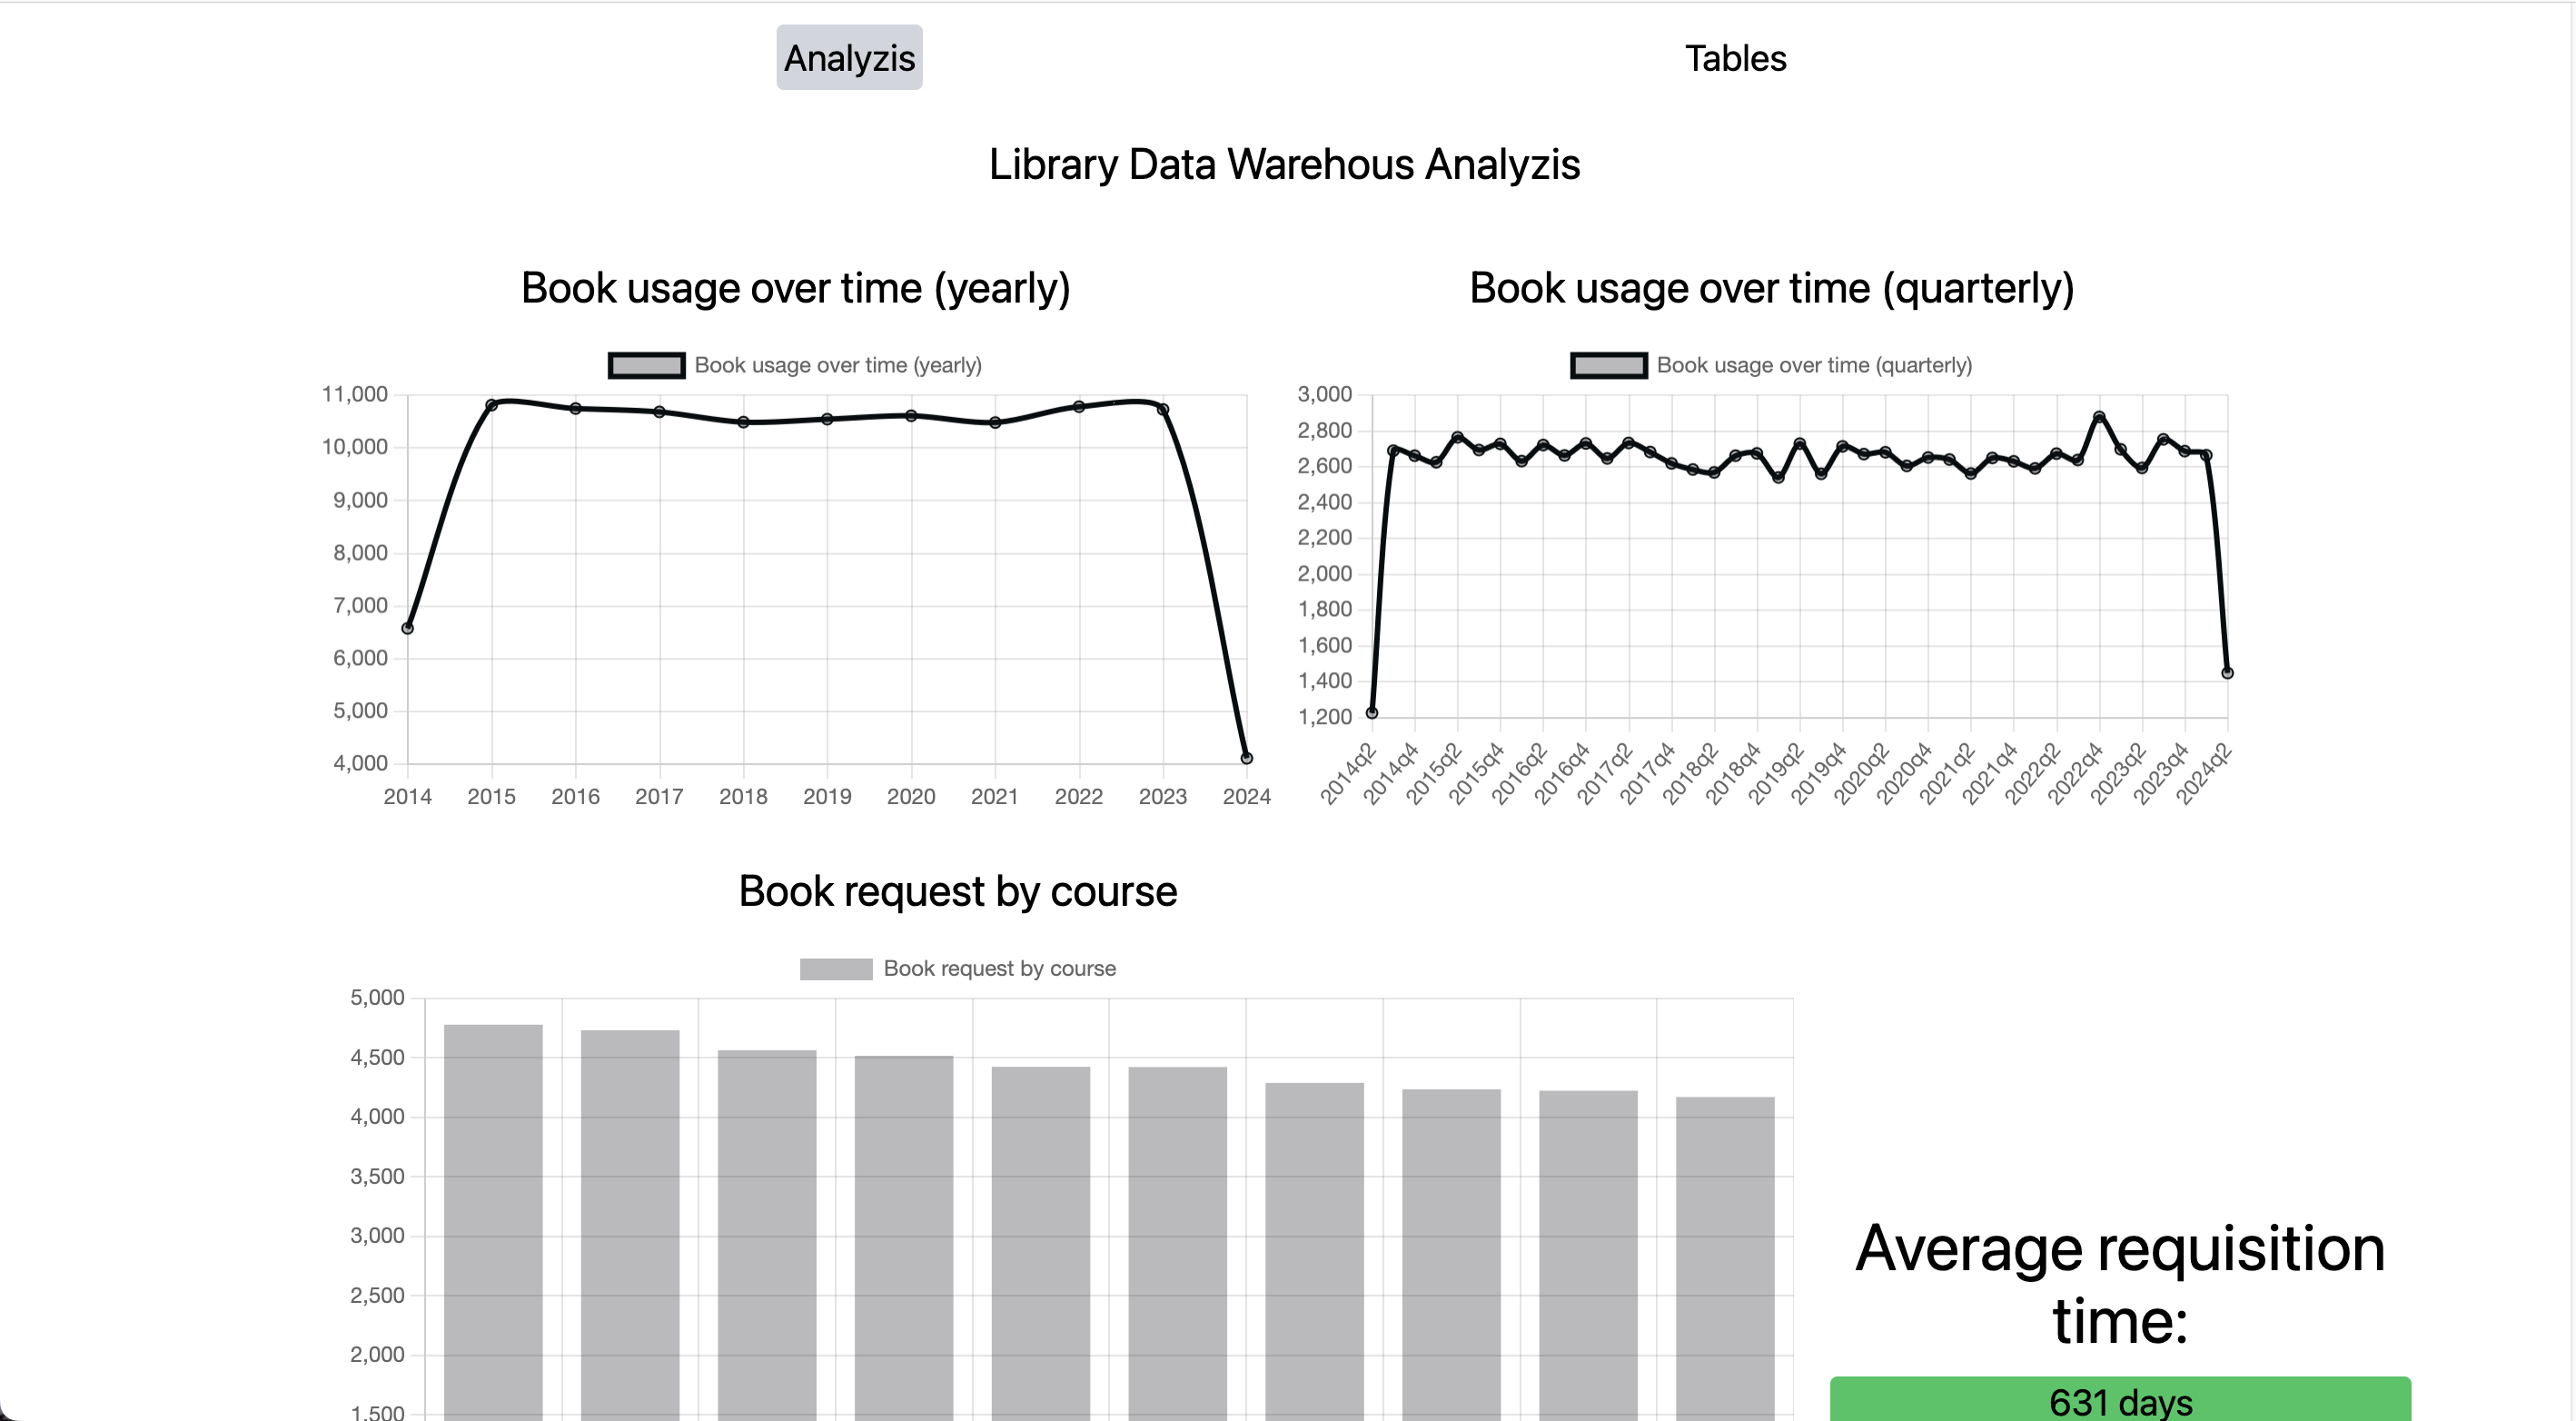
\includegraphics[width=0.95\textwidth]{figures/frontend.png}
    \end{center}
    \caption{Frontend Index Page}\label{fig:frontend}
\end{figure}


\chapter{Conclusion} % (fold)
\label{chap:Conclusion}

In conclusion, this final project for the data warehouses class has been an enlightening experience in navigating various obstacles, both expected and unexpected. As an Erasmus student, the lack of an English translation for the task presented an initial challenge that I had to overcome with the aid of Google Translate. This added an unnecessary layer of complexity to an already demanding project.

The Radzen tool we were required to use was, to put it mildly, less than ideal. Its functionality was limited, and it frequently failed to work as intended. This significantly hampered the development process and increased the time and effort required to complete even basic tasks.

The data provided for this project was another source of frustration. The request.csv and books.csv files contained book IDs that were disjoint, making it impossible to match requests to actual books. This fundamental flaw suggests that the data was likely auto-generated without proper validation or consideration for practical usability. Consequently, any conclusions drawn from this data are, at best, questionable and, at worst, completely meaningless.

Despite these challenges, I endeavored to create a data warehouse that could potentially serve as a foundation for analyzing library data over the past ten years. However, the inherent flaws in the data and tools provided mean that the insights and conclusions derived from this project should be taken with a grain of salt.

Overall, this project has highlighted the importance of reliable tools, accurate data, and clear communication in the development of a functional data warehouse. It has been an exercise in patience and problem-solving under less-than-ideal circumstances, and while the final product may not meet the intended objectives, it stands as a testament to the resilience and resourcefulness required to navigate such a flawed assignment.


% chapter Conclusion (end)



\appendix
\chapter{Codes}
\label{appendix:codes}

\section{Transform Script}
\label{appendix:transform_script}

\begin{lstlisting}[language=python, caption={Transform script}, label={lst:transform_script}]
import pandas as pd


def get_max_len(lista):
    return max(list(map(lambda x: (len(x)), lista)))


csv_path = "../data_csv/"
dest_path = "../data_transformed/"


book_file = "book.csv"
student_file = "student.csv"
request_file = "request.csv"
resident_file = "population.csv"

book_usecols = ["book_id", "title", "price", "purchase_date", "availability"]
book = pd.read_csv(csv_path + book_file, index_col="book_id", usecols=book_usecols)
print(f'max book.title length: { get_max_len(book["title"].values) }')

student_usecols = ["student_id", "name", "course", "address", "gender", "date_of_birth"]
student = pd.read_csv(csv_path + student_file, index_col="student_id", usecols=student_usecols)
print(f'max student.course length: { get_max_len(student["course"].values) }')
print(f'max student.address length: { get_max_len(student["address"].values) }\n')
print(f'max student.name length: { get_max_len(student["name"].values) }\n')

request = pd.read_csv(csv_path + request_file, index_col="request_id")

population = pd.read_csv(csv_path + resident_file, index_col="population_id")
print(f'max population.city length: { get_max_len(population["city"].values) }')
print(f'max population.region_type length: { get_max_len(population["region_type"].values) }')




def save():
    population.to_csv(dest_path + resident_file)
    book.to_csv(dest_path + book_file)
    request.to_csv(dest_path + request_file)
    student.to_csv(dest_path + student_file)


save()
\end{lstlisting}

\section{SQL} 
\label{appendix:init_sql}


\begin{lstlisting}[language=SQL, caption={init.sql}, label={lst:init_sql}]
DROP TABLE IF EXISTS fact_request;

DROP TABLE IF EXISTS dim_student;
CREATE TABLE dim_student
(
    student_id INT NOT NULL,
    name VARCHAR(27) NOT NULL,
    course VARCHAR(87) NOT NULL,
    gender VARCHAR(1) NOT NULL,
    date_of_birth DATE NOT NULL,
    address VARCHAR(79) NOT NULL,
    PRIMARY KEY (student_id)
);

CREATE INDEX d_student_int_student_id_idx ON dim_student(student_id);

-------------------------------

DROP TABLE IF EXISTS dim_book;
CREATE TABLE dim_book
(
    book_id INT NOT NULL,
    title VARCHAR(59) NOT NULL,
    availability BOOLEAN NOT NULL,
    purchase_date DATE NOT NULL,
    price FLOAT NOT NULL,
    PRIMARY KEY (book_id)
);
CREATE INDEX d_book_id_idx ON dim_book(book_id);

-------------------------------

DROP TABLE IF EXISTS dim_population;
CREATE TABLE dim_population
(
    population_id INT NOT NULL,
    city VARCHAR(28) NOT NULL,
    region_type VARCHAR(9) NOT NULL,
    population INT NOT NULL,
    PRIMARY KEY (population_id)
);
CREATE INDEX d_population_id_idx ON dim_population(population_id);

-------------------------------

DROP TABLE if exists dim_date;
CREATE TABLE dim_date
(
    -- loan_date_id              INT NOT NULL,
    date_actual              DATE NOT NULL,
    epoch                    BIGINT NOT NULL,
    day_name                 VARCHAR(9) NOT NULL,
    day_of_week              INT NOT NULL,
    day_of_month             INT NOT NULL,
    day_of_quarter           INT NOT NULL,
    day_of_year              INT NOT NULL,
    week_of_month            INT NOT NULL,
    week_of_year             INT NOT NULL,
    week_of_year_iso         CHAR(10) NOT NULL,
    month_actual             INT NOT NULL,
    month_name               VARCHAR(9) NOT NULL,
    month_name_abbreviated   CHAR(3) NOT NULL,
    quarter_actual           INT NOT NULL,
    quarter_name             VARCHAR(9) NOT NULL,
    year_actual              INT NOT NULL,
    first_day_of_week        DATE NOT NULL,
    last_day_of_week         DATE NOT NULL,
    first_day_of_month       DATE NOT NULL,
    last_day_of_month        DATE NOT NULL,
    first_day_of_quarter     DATE NOT NULL,
    last_day_of_quarter      DATE NOT NULL,
    first_day_of_year        DATE NOT NULL,
    last_day_of_year         DATE NOT NULL,
    mmyyyy                   CHAR(6) NOT NULL,
    mmddyyyy                 CHAR(10) NOT NULL,
    weekend_indr             BOOLEAN NOT NULL,
    PRIMARY KEY (date_actual)
);
CREATE INDEX d_loan_date_date_actual_idx ON dim_date(date_actual);

-------------------------------

CREATE TABLE stage_request
(
    request_id INT NOT NULL,
    student_id INT NOT NULL,
    book_id INT NOT NULL,
    loan_date DATE NOT NULL,
    PRIMARY KEY (request_id)
);

-------------------------------

INSERT INTO dim_date
    SELECT --TO_CHAR(datum, 'yyyymmdd')::INT AS date_id,
        datum AS date_actual,
        EXTRACT(EPOCH FROM datum) AS epoch,
        TO_CHAR(datum, 'TMDay') AS day_name,
        EXTRACT(ISODOW FROM datum) AS day_of_week,
        EXTRACT(DAY FROM datum) AS day_of_month,
        datum - DATE_TRUNC('quarter', datum)::DATE + 1 AS day_of_quarter,
        EXTRACT(DOY FROM datum) AS day_of_year,
        TO_CHAR(datum, 'W')::INT AS week_of_month,
        EXTRACT(WEEK FROM datum) AS week_of_year,
        EXTRACT(ISOYEAR FROM datum) || TO_CHAR(datum, '"-W"IW-') || EXTRACT(ISODOW FROM datum) AS week_of_year_iso,
        EXTRACT(MONTH FROM datum) AS month_actual,
        TO_CHAR(datum, 'TMMonth') AS month_name,
        TO_CHAR(datum, 'Mon') AS month_name_abbreviated,
        EXTRACT(QUARTER FROM datum) AS quarter_actual,
        CASE
            WHEN EXTRACT(QUARTER FROM datum) = 1 THEN 'First'
            WHEN EXTRACT(QUARTER FROM datum) = 2 THEN 'Second'
            WHEN EXTRACT(QUARTER FROM datum) = 3 THEN 'Third'
            WHEN EXTRACT(QUARTER FROM datum) = 4 THEN 'Fourth'
        END AS quarter_name,
        EXTRACT(YEAR FROM datum) AS year_actual,
        datum + (1 - EXTRACT(ISODOW FROM datum))::INT AS first_day_of_week,
        datum + (7 - EXTRACT(ISODOW FROM datum))::INT AS last_day_of_week,
        datum + (1 - EXTRACT(DAY FROM datum))::INT AS first_day_of_month,
        (DATE_TRUNC('MONTH', datum) + INTERVAL '1 MONTH - 1 day')::DATE AS last_day_of_month,
        DATE_TRUNC('quarter', datum)::DATE AS first_day_of_quarter,
        (DATE_TRUNC('quarter', datum) + INTERVAL '3 MONTH - 1 day')::DATE AS last_day_of_quarter,
        TO_DATE(EXTRACT(YEAR FROM datum) || '-01-01', 'YYYY-MM-DD') AS first_day_of_year,
        TO_DATE(EXTRACT(YEAR FROM datum) || '-12-31', 'YYYY-MM-DD') AS last_day_of_year,
        TO_CHAR(datum, 'mmyyyy') AS mmyyyy,
        TO_CHAR(datum, 'mmddyyyy') AS mmddyyyy,
        CASE
            WHEN EXTRACT(ISODOW FROM datum) IN (6, 7) THEN TRUE
            ELSE FALSE
        END AS weekend_indr
    FROM (SELECT '2014-05-21'::DATE + SEQUENCE.DAY AS datum
        FROM GENERATE_SERIES(0, 3654) AS SEQUENCE (DAY)
        GROUP BY SEQUENCE.DAY) DQ
    ORDER BY 1;

-------------------------------

CREATE TABLE fact_request
(
    request_id INT NOT NULL,
    loan_date DATE NOT NULL,
    student_id INT NOT NULL,
    book_id INT NOT NULL,
    population_id INT,
    -- PRIMARY KEY (request_id),
    FOREIGN KEY (student_id) REFERENCES dim_student(student_id),
    FOREIGN KEY (book_id) REFERENCES dim_book(book_id),
    FOREIGN KEY (population_id) REFERENCES dim_population(population_id),
    FOREIGN KEY (loan_date) REFERENCES dim_date(date_actual)
);

-------------------------------

COPY dim_book
FROM '/data/book.csv'
DELIMITER ','
CSV HEADER;

COPY dim_student
FROM '/data/student.csv'
DELIMITER ','
CSV HEADER;

COPY dim_population
FROM '/data/population.csv'
DELIMITER ','
CSV HEADER;

COPY stage_request
FROM '/data/request.csv'
DELIMITER ','
CSV HEADER;



insert into fact_request 
    select request_id, loan_date, sr.student_id, sr.book_id, dp.population_id
    from dim_population dp, stage_request sr
    inner join 
    dim_student ds
    on ds.student_id = sr.student_id
    inner join
    dim_book dib
    on dib.book_id = sr.book_id
    inner join
    dim_date dd
    on dd.date_actual = sr.loan_date
    where ds.address like '%' || dp.city || '%'
    order by loan_date;

drop table if exists stage_request;


--------------------------------------------------------------------
--------------------------- SOLUTIONS ------------------------------
--------------------------------------------------------------------

--- gettin the average request time
create or replace view avg_time as
WITH next_loan AS (
    SELECT 
        request_id,
        student_id,
        book_id,
        loan_date,
        LEAD(loan_date) OVER (PARTITION BY book_id ORDER BY loan_date) AS next_loan_date
    FROM 
        fact_request
)
SELECT 
    AVG(next_loan_date - loan_date) AS average_requisition_time
FROM 
    next_loan
WHERE 
    next_loan_date IS NOT NULL;

-------------------------------------------------------------------
--- book usage over time yearly

create or replace view usage_year as
SELECT
    dd.year_actual as first,
    COUNT(fr.request_id) AS second
FROM
    fact_request fr
JOIN
    dim_date dd ON fr.loan_date = dd.date_actual
GROUP BY
    dd.year_actual
ORDER BY
    year_actual;

-------------------------------------------------------------------
--- book usage over time quarterly
create or replace view usage_quarter as
SELECT
    dd.year_actual,
    dd.quarter_actual,
    COUNT(fr.request_id) AS total_loans
FROM
    fact_request fr
JOIN
    dim_date dd ON fr.loan_date = dd.date_actual
GROUP BY
    dd.year_actual,
    dd.quarter_actual
ORDER BY
    dd.year_actual,
    dd.quarter_actual;

--- book usage over time montly
create or replace view usage_month as
SELECT
    dd.year_actual,
    dd.month_actual,
    COUNT(fr.request_id) AS total_loans
FROM
    fact_request fr
JOIN
    dim_date dd ON fr.loan_date = dd.date_actual
GROUP BY
    dd.year_actual,
    dd.month_actual
ORDER BY
    dd.year_actual,
    dd.month_actual;


-------------------------------------------------------------------
---books that have never been requested, and their associated costs.
create or replace view never_requested as
select dim_book.title as title, dim_book.price as price
	from dim_book
	where book_id not in (select book_id from fact_request)
	order by price desc
	offset 0
    fetch next 50 rows only;

-------------------------------------------------------------------
---Identify which city have the most readers
create or replace view most_reader_city as
select dim_population.city as first, count(request_id) as second from fact_request
inner join
dim_population on dim_population.population_id = fact_request.population_id
group by dim_population.population_id
order by second desc;



-------------------------------------------------------------------
--- the most requested books per:
-- student
create or replace view most_request_student as
WITH student_book_requests AS (
    SELECT
        fr.student_id,
        fr.book_id,
        COUNT(fr.request_id) AS request_count
    FROM
        fact_request fr
    GROUP BY
        fr.student_id,
        fr.book_id
),
ranked_books AS (
    SELECT
        sbr.student_id,
        sbr.book_id,
        sbr.request_count,
        ROW_NUMBER() OVER (PARTITION BY sbr.student_id ORDER BY sbr.request_count DESC) AS rank
    FROM
        student_book_requests sbr
)
SELECT
    ds.name,
    db.title,
    rb.request_count
FROM
    ranked_books rb
JOIN
    dim_student ds ON rb.student_id = ds.student_id
JOIN
    dim_book db ON rb.book_id = db.book_id
WHERE
    rb.rank = 1
ORDER BY
    rb.request_count desc;


-- per course
create or replace view most_request_course as
WITH course_book_requests AS (
    SELECT
        ds.course,
        fr.book_id,
        COUNT(fr.request_id) AS request_count
    FROM
        fact_request fr
    JOIN
        dim_student ds ON fr.student_id = ds.student_id
    GROUP BY
        ds.course,
        fr.book_id
),
ranked_books AS (
    SELECT
        cbr.course,
        cbr.book_id,
        cbr.request_count,
        ROW_NUMBER() OVER (PARTITION BY cbr.course ORDER BY cbr.request_count DESC) AS rank
    FROM
        course_book_requests cbr
)
SELECT
    rb.course,
    db.title
    -- rb.request_count
FROM
    ranked_books rb
JOIN
    dim_book db ON rb.book_id = db.book_id
WHERE
    rb.rank = 1
ORDER BY
    rb.course;

create view request_course as
SELECT ds.course, COUNT(fr.request_id) AS count FROM fact_request fr JOIN dim_student ds ON fr.student_id = ds.student_id GROUP BY ds.course ORDER BY count DESC LIMIT 10; 

-- by gender
create or replace view most_request_gender as
select dim_student.gender as gender, dim_book.title from fact_request
inner join
dim_student on dim_student.student_id = fact_request.student_id
inner join
dim_book on dim_book.book_id = fact_request.book_id
group by dim_student.gender, title
	order by count(request_id) desc;



-- by districts with higher populations
create or replace view most_request_population as
select dim_population.city as first, count(request_id) as second
	from fact_request
	join
	dim_population on dim_population.population_id = fact_request.population_id
	where dim_population.population > 250000
	group by dim_population.city
	order by second desc;


-------------------------------------------------------------------
--- Analyze annual acquisition costs 
create or replace view an_annual_cost as
SELECT
    EXTRACT(YEAR FROM purchase_date) AS purchase_year,
    SUM(price) AS total_acquisition_cost
FROM
    dim_book
GROUP BY
    purchase_year
ORDER BY
    purchase_year;


-------------------------------------------------------------------
--- Analyze the relationship between reading newer and older books
create or replace view an_new_old as
SELECT
    EXTRACT(YEAR FROM fr.loan_date) AS loan_year,
    CASE
        WHEN AGE(fr.loan_date, db.purchase_date) <= INTERVAL '1 year' THEN '0-1 year'
        WHEN AGE(fr.loan_date, db.purchase_date) <= INTERVAL '2 year' THEN '1-2 years'
        WHEN AGE(fr.loan_date, db.purchase_date) <= INTERVAL '5 year' THEN '2-5 years'
        ELSE '5+ years'
    END AS book_age_category,
    COUNT(fr.request_id) AS total_requests
FROM
    fact_request fr
JOIN
    dim_book db ON fr.book_id = db.book_id
GROUP BY
    loan_year,
    book_age_category
ORDER BY
    loan_year,
    book_age_category;

-------------------------------------------------------------------
--- books not returned, among other aspects
create or replace view not_returned as
with next_loan as ( SELECT 
        request_id,
        student_id,
        book_id,
        loan_date,
        LEAD(loan_date) OVER (PARTITION BY book_id ORDER BY loan_date) AS next_loan_date
    FROM 
        fact_request
) select dim_book.book_id, title from next_loan
	inner join
	dim_book on dim_book.book_id = next_loan.book_id
	where next_loan_date is null
	group by dim_book.book_id;

-------------------------------------------------------------------
--- Determine the busiest day of the week for requisitions on average
create or replace view busy_day as
SELECT
    dd.day_name,
    COUNT(fr.request_id) AS total_requests
FROM
    fact_request fr
JOIN
    dim_date dd ON fr.loan_date = dd.date_actual
GROUP BY
    dd.day_name
ORDER BY
    total_requests DESC;

-------------------------------------------------------------------
--- Determine the months with the highest usage.
create or replace view busy_month as
SELECT
    dd.month_name,
    COUNT(fr.request_id) AS total_requests
FROM
    fact_request fr
JOIN
    dim_date dd ON fr.loan_date = dd.date_actual
GROUP BY
    dd.month_name, 
    dd.month_actual
ORDER BY
    total_requests desc;

\end{lstlisting}


% \printbibliography
% \addcontentsline{toc}{chapter}{References}


\end{document}
